\documentclass{beamer}
\usepackage[utf8]{inputenc}
\usepackage{graphicx}
\usepackage{color}
%\usetheme{Hannover}
\newcommand{\hilight}[1]{\textbf{\textcolor{structure.fg!85}{#1}}}
\setbeamertemplate{footline}[frame number]

\usepackage{hyperref}
\hypersetup{
    colorlinks=true,
    linkcolor=blue,
    filecolor=magenta,      
    urlcolor=cyan,
}

\author[Sowmya Vajjala]{Sowmya Vajjala}

\title[SfSNLP]{NLP without Annotated Dataset}
\subtitle{Text Embeddings and Transfer Learning in NLP}


\date{20 January 2021}

\institute{Seminar f\"ur Sprachwissenschaft, University of T\"ubingen, Germany}
%%%%%%%%%%%%%%%%%%%%%%%%%%%

\begin{document}

\begin{frame}\titlepage
\end{frame}

\begin{frame}{Class Outline}
    \begin{itemize}
        \item Reminders + Last class - a quick recap
        \item Text representation - a quick recap
        \item Neural text embedding -word2vec to BERTs: an overview
        \item Using embeddings for downstream NLP tasks: examples
        \item Transfer learning for NLP: an example with Fine-Tuning BERT
        \end{itemize}
        
        Note: This is perhaps going to be a long expository session. Be prepared!
\end{frame}

\begin{frame}
\frametitle{Group Discussion schedule}
\begin{itemize}
\item We are starting this Friday!
    \item Teams/Papers info on the forum.
    \item Presentation schedule  (also posted on forum)
    \begin{enumerate}
        \item 22nd January: Teams 1--3
        \item 25th January: Teams 4--6
        \item 27th January: Teams 7--9
    \end{enumerate}
    \item Format: 15-20 minutes of presentation, Around 10 min of discussion per team (everyone can ask questions. Presenters don't have to know all answers. I will also try to answer some of the questions that come up!)
\end{itemize}
Questions on this? 
\end{frame}


\begin{frame}
\frametitle{Last Class}
\begin{itemize}
\item Spam classification with snorkel:
\begin{itemize}
    \item Data labeling with labeling functions
    \item Data augmentation with transformation functions
    \item How do they both compare with the original training data (with labels)
\end{itemize}
\end{itemize}
- Questions or comments on this? 
\end{frame}

\begin{frame}{Text Representation: A quick recap}
\begin{itemize}
    \item Bag of words
    \item Bag of n-grams
    \item TF-IDF
\end{itemize}
note: code examples in following slides taken from Chapter 3 of Practical NLP Book. \href{https://github.com/practical-nlp/practical-nlp/tree/master/Ch3}{(github repo)}
\end{frame}

\begin{frame}
\frametitle{Words and Vectors}
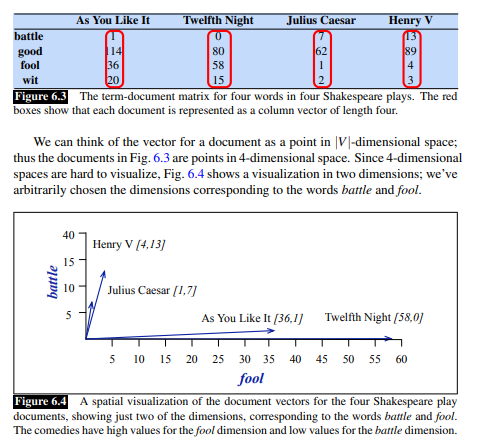
\includegraphics[width=0.8\textwidth]{figures/wordsvectors1.PNG}
\\ \tiny source: \url{https://web.stanford.edu/~jurafsky/slp3/6.pdf}
\end{frame}

\begin{frame}
\frametitle{Bag of Words}
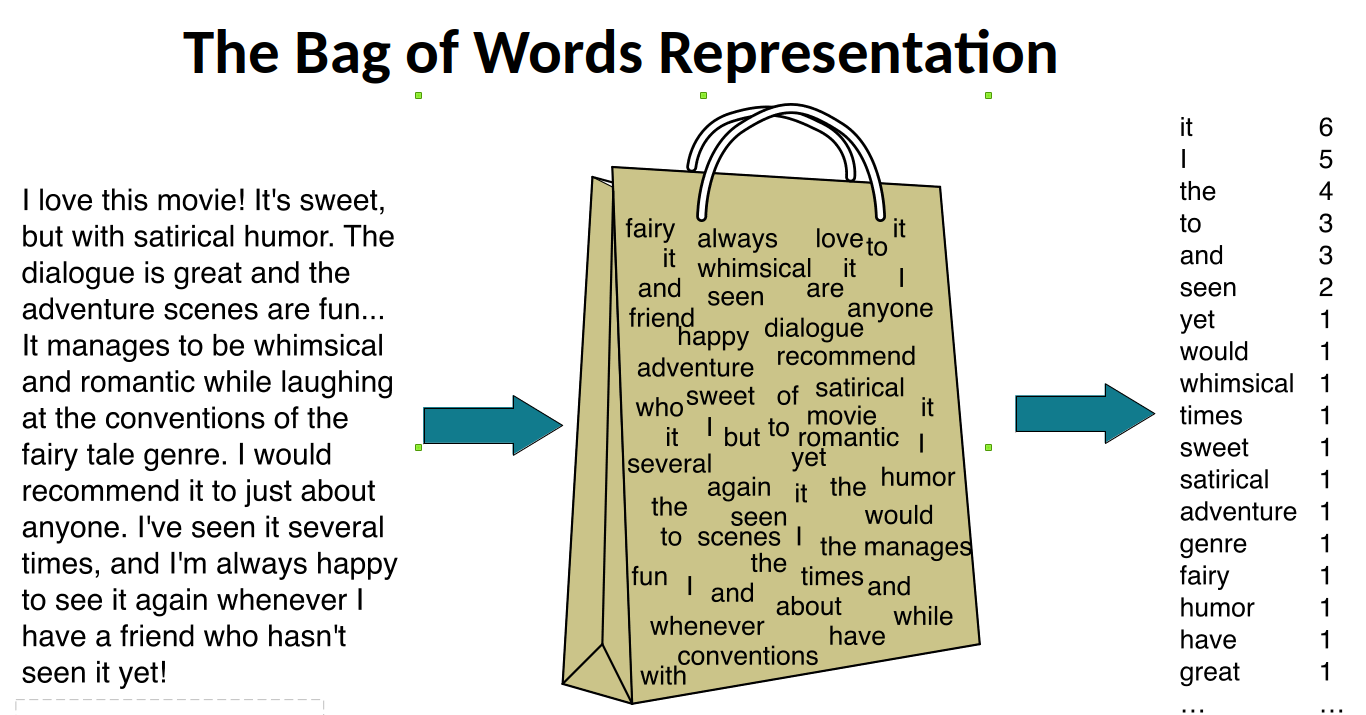
\includegraphics[width=0.9\textwidth]{figures/bow.png}
\\ \tiny source: \url{https://web.stanford.edu/~jurafsky/slp3/4.pdf}
\end{frame}

\begin{frame}[fragile]{Toy Corpus}
\small
    \begin{verbatim}
    documents = ["Dog bites man.", "Man bites dog.", 
                "Dog eats meat.", "Man eats food."] 
    processed_docs = [doc.lower().replace(".","") 
                      for doc in documents]
    print(processed_docs)
    \end{verbatim}
    
    \footnotesize     
    output: $[$ 'dog bites man', 'man bites dog', 'dog eats meat', 'man eats food'$]$
\end{frame}

\begin{frame}
\frametitle{BOW Example}
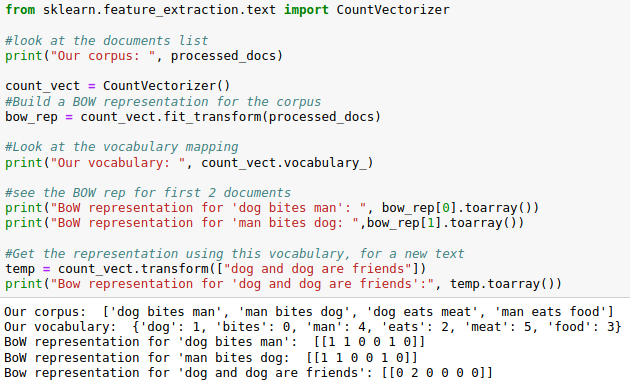
\includegraphics[width=0.8\textwidth]{figures/bowexample.png}
\end{frame}

\begin{frame}
\frametitle{BOW Example with Binary Values}
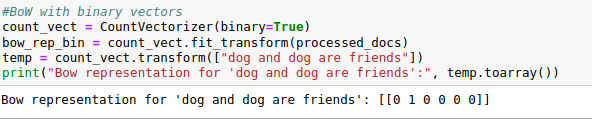
\includegraphics[width=\textwidth]{figures/bowbinaryrep.png}
\end{frame}

\begin{frame}
\frametitle{BON Example}
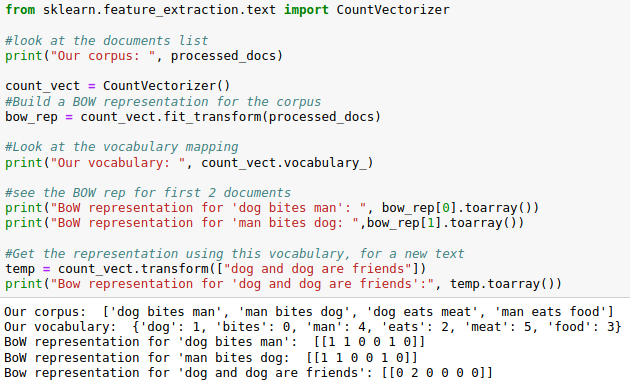
\includegraphics[width=\textwidth]{figures/bowexample.png}
\end{frame}

\begin{frame}
\frametitle{TF-IDF}
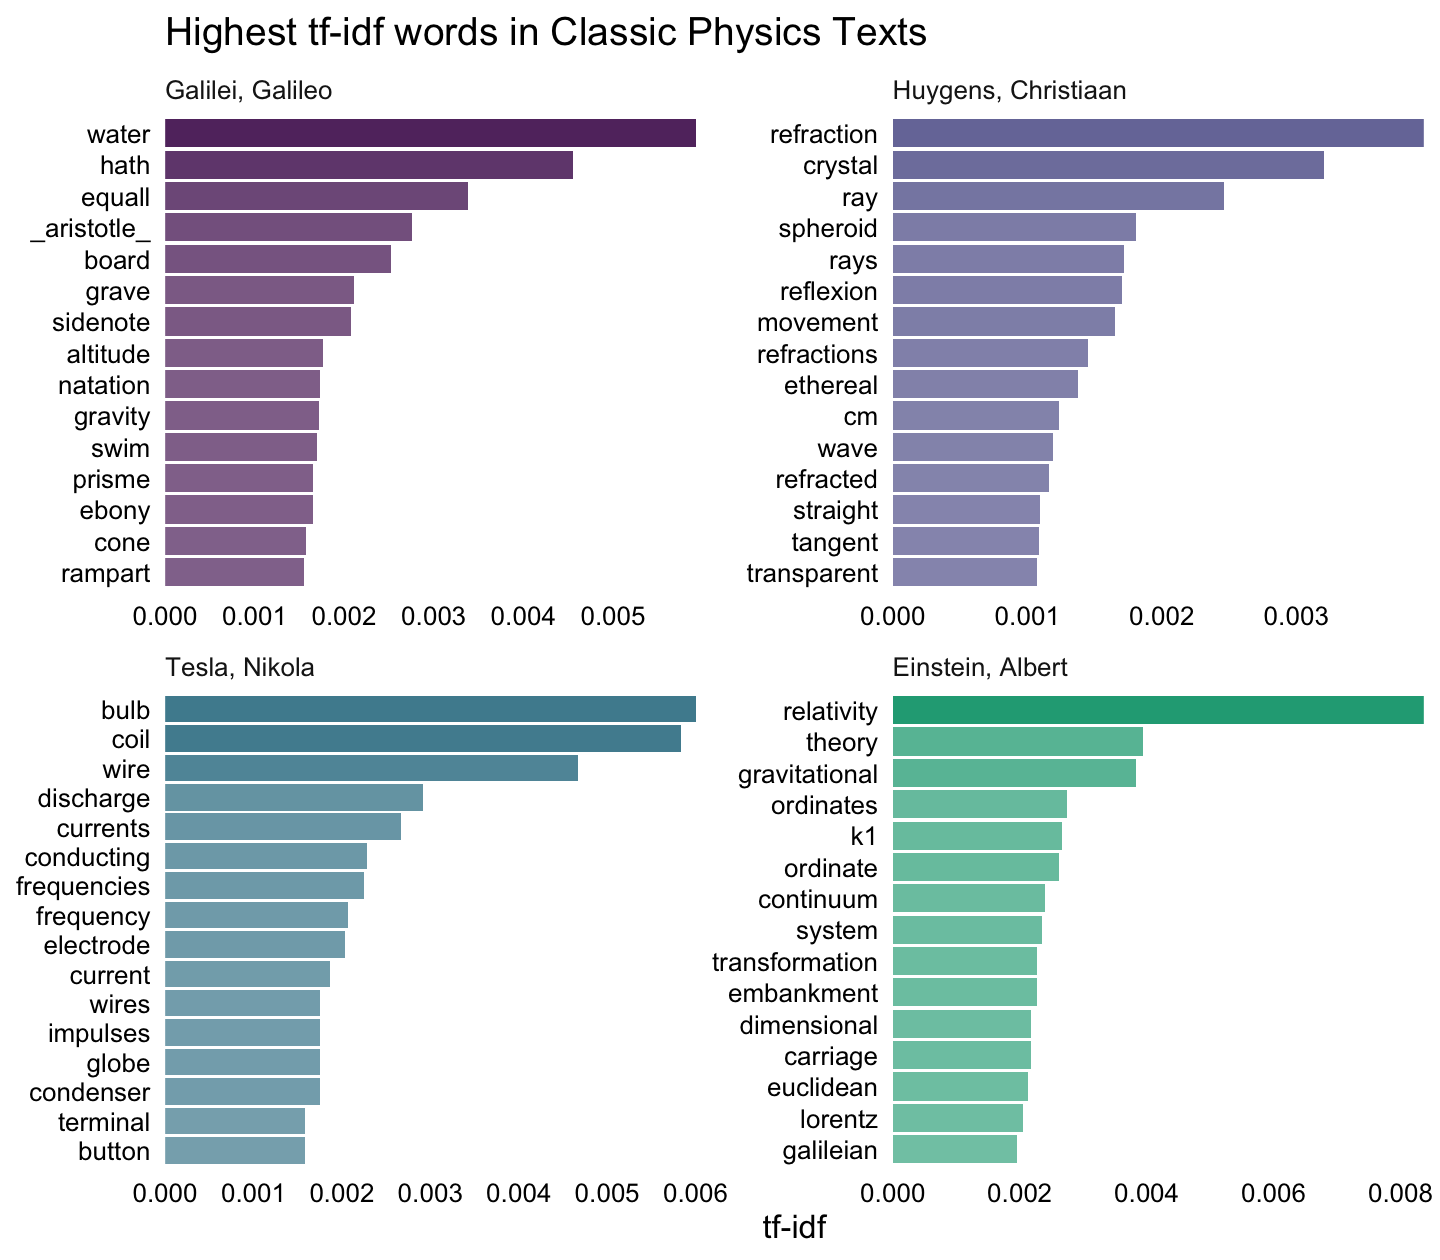
\includegraphics[width=0.8\textwidth]{figures/tfidfpic.png}
\\ \tiny source: \url{https://www.r-bloggers.com/2016/06/term-frequency-and-tf-idf-using-tidy-data-principles/}
\end{frame}

\begin{frame}
\frametitle{TF-IDF Example}
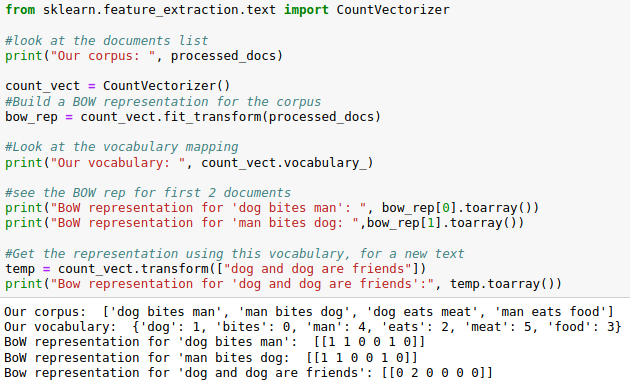
\includegraphics[width=\textwidth]{figures/bowexample.png}
\end{frame}

\begin{frame}{What is good about these representations?}
    \begin{itemize}
        \item Easy to understand.
        \item Easy to implement programmatically.
        \item Documents sharing vocabulary will be close to each other in the representation space.
        \item We have a fixed length vector for a sentence/text of any length. (What does this mean?)
    \end{itemize}
\end{frame}

\begin{frame}{What are some drawbacks?}
    \begin{itemize}
        \item Size of the vector: If we take Bag of Words/TF-IDF, it is the number of unique words in the corpus. If we take N-grams, it is the number of unique n-grams. 
        \\ $\Rightarrow$ This can get pretty big (unless we decide to cut it at top-N words/ngrams).
        \item Most of the items in the vector are zeroes (so, these vectors are sparse) - why is this a problem? \pause
        \item If we encounter a new word later while using this representation on new texts, we don't know what to do. \pause
    \end{itemize}
    -  How do we address these issues? \pause Text embeddings are a step in that direction. 
\end{frame}

\begin{frame}{Before learning about embeddings...}
\framesubtitle{Distributional Hypothesis}
    \begin{itemize}
        \item Words that occur in similar contexts may be related in some way (synonyms, antonyms etc)
        \item The link between similarity in how words are distributed and similarity
in what they mean is called the distributional hypothesis.
\item This hypothesis was studied in 20th century linguistics in 1950s and it extended to the concept of "vector semantics" which forms the basis of neural text representations known as embeddings in NLP. 
    \end{itemize}
    
    Slides that follow are based on Chapter 6 in Jurafsky \& Martin, 3rd Edition 
\end{frame}

\begin{frame}
\frametitle{Words and their relationships}
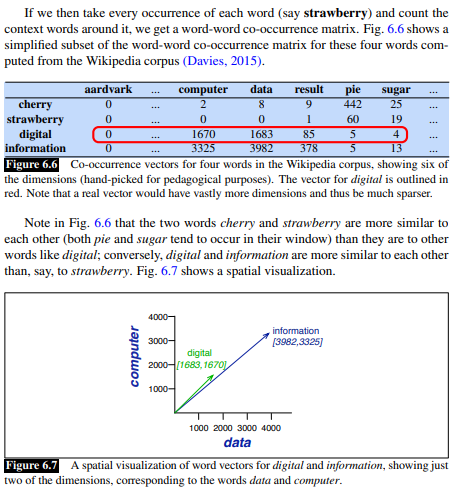
\includegraphics[width=0.7\textwidth]{figures/wordsvectors2.PNG}
\\ \tiny source: \url{https://web.stanford.edu/~jurafsky/slp3/6.pdf}
\end{frame}

\begin{frame}
\frametitle{Similarity between two words}
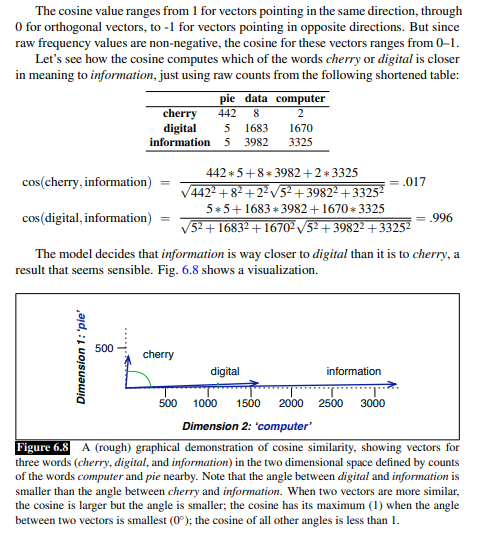
\includegraphics[width=0.7\textwidth]{figures/cosine.PNG}
\\ \tiny source: \url{https://web.stanford.edu/~jurafsky/slp3/6.pdf}
\end{frame}

\begin{frame}{Intuition}
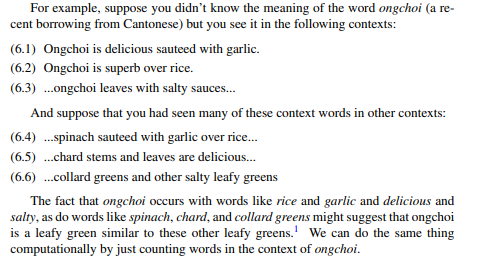
\includegraphics[width=\textwidth]{figures/ongchoi.PNG}
\\ \tiny source: \url{https://web.stanford.edu/~jurafsky/slp3/6.pdf}
\end{frame}

\begin{frame}{Vector Semantics}
    \begin{itemize}
        \item Vector semantics is the standard way to represent word meaning in NLP.
        \item Vector semantic approaches "learn" to define the meaning of a word by its distribution in language use i.e., its neighboring words or grammatical environment. \pause
        \item The goal of such a model is to represent a word as a point in a multidimensional semantic space (called an "embedding") that is derived from distributions of its neighbors.
        \item The question of how to "learn" this multidimensional space resulted in various approaches to word embeddings in NLP.
    \end{itemize}
\end{frame}

\begin{frame}{What do Embeddings learn?}
    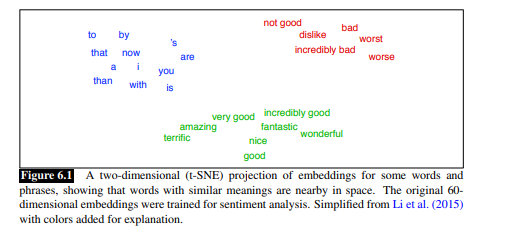
\includegraphics[width=\textwidth]{figures/embeddingsvisualization.PNG}
\\ \tiny source: \url{https://web.stanford.edu/~jurafsky/slp3/6.pdf}
\end{frame}

\begin{frame}{Earlier text representations vs embeddings} %TODO!
    \begin{itemize}
        \item Count based vs learnt representations
        \item Sparse vectors with mostly zeros vs Dense vectors with non-zero values in all dimensions. 
        \item Long vectors, scaling with vocabulary size vs Short vectors with limited dimensions. 
    \end{itemize}
\end{frame}

\begin{frame}{Why bother about embeddings?}
    \begin{itemize}
        \item Because embeddings are everywhere now!
        \item It turns out that dense vectors typically work better in every NLP task than sparse vectors. \pause
        \item Although we don't fully know why yet, it is possible that:
        \begin{itemize}
            \item Shorter and denser vectors will need fewer parameters to learn better for ML/DL models.
            \item Dense vectors may be capturing synonymy and other relations between words. 
        \end{itemize}
    \end{itemize}
\end{frame}

\begin{frame}{Text Embeddings: Word2Vec} 
\begin{itemize}
    \item Intuition: instead of counting how often each word w occurs near, say, apricot, we’ll train a classifier on a binary prediction task: “Is word w likely to show up near apricot?”  \pause
    \item We don’t actually care about this prediction task; instead we’ll take the learned classifier weights as the word embeddings. \pause
    \item The revolutionary intuition here is that we can just use running text as implicitly
supervised training data for such a classifier;
\item a word c that occurs near the target word apricot acts as gold ‘correct answer’ to the question “Is word c likely to show up near apricot?” 
\item This method, often called self-supervision, avoids the need for any sort of hand-labeled supervision signal.
\end{itemize}
\end{frame}

\begin{frame}{How do we use them?}
\begin{itemize}
    \item Pre-trained word2vec embeddings are available for various kinsd of text.
    \item If you want to train your own word2vec embeddings for a specific problem domain, it is easy and fast.
    \item Instead of using bag of words/ngrams etc, you can just use them as features.
    \item How?: A common strategy is to get embeddings for individual words from this model, and average them to get full text feature representation
\end{itemize}
\end{frame}

\begin{frame}[fragile]{Using pre-trained word2vec}
\tiny
    \begin{verbatim}
        from gensim.models import Word2Vec, KeyedVectors
        pretrainedpath = '/tmp/input/GoogleNews-vectors-negative300.bin.gz'
        w2v_model = KeyedVectors.load_word2vec_format(pretrainedpath, binary=True) 
        #loads the model
    
        #What is the vector representation for a word? 
        w2v_model['computer']
    \end{verbatim}
    \\ \href{https://github.com/practical-nlp/practical-nlp/blob/master/Ch3/05_Pre_Trained_Word_Embeddings.ipynb}{source}

\end{frame}

\begin{frame}[fragile]{Training a word2vec model}
\tiny
    \begin{verbatim}
from gensim.test.utils import common_texts
from gensim.models import Word2Vec
model = Word2Vec(sentences=common_texts, vector_size=100, window=5, min_count=1, workers=4)
model.save("word2vec.model")
    \end{verbatim}
    More details: \url{https://radimrehurek.com/gensim/models/word2vec.html}
\end{frame}

\begin{frame}{What do Embeddings learn?}
    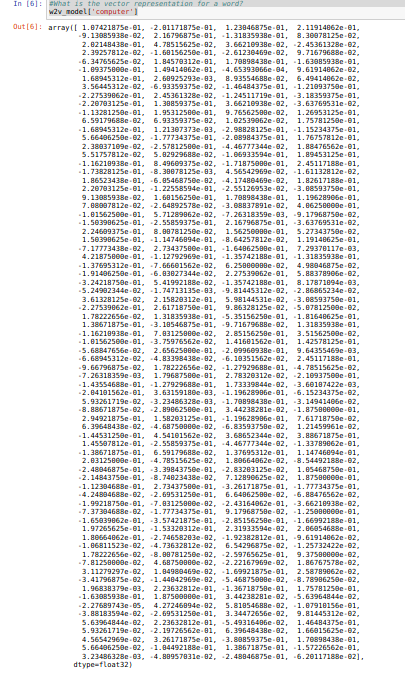
\includegraphics[width=\textwidth]{figures/w2vrep.png}
\end{frame}

\begin{frame}{What does word2vec learn?}
\framesubtitle{A small exercise}
    Go to: \url{http://bionlp-www.utu.fi/wv_demo/} and explore the interface with the English word2vec model provided (10 minutes). Share your observations on what the model does afterwards.
\end{frame}

\begin{frame}{}
    \large Share your observations.
\end{frame}

\begin{frame}{How to get from word to document?}
    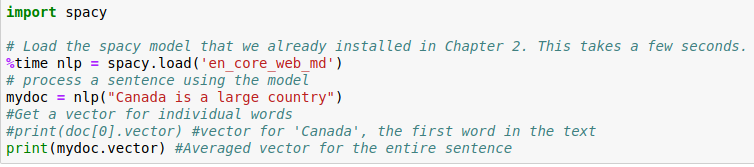
\includegraphics[width=\textwidth]{figures/w2vavged.png}
\end{frame}

\begin{frame}{Out of vocabulary words}
What do we do when we encounter a new word not seen in the training vocabulary?
        \begin{itemize}
            \item Leave it out of your feature vector calculation for the text (a common strategy)
            \item Randomly initialize a vector
            \item "Learn" a representation for a OOV word by randomly replacing words during training with a new word token. 
            \item ....
    \end{itemize}
\end{frame}
    
\begin{frame}{A better way: FastText embeddings}
    \begin{itemize}
        \item FastText deals with unknown words and sparsity in languages with rich morphology, by using subword models. 
        \item Each word in fasttext is represented as itself plus a bag of constituent n-grams, with special boundary symbols $<$ and $>$ added to each word.
        \item For example, with n = 3 the word where would be represented by the sequence <where> plus the character n-grams: $<$wh, whe, her, ere, re$>$
        \item Then an embedding is learned for each constituent n-gram (instead of words themselves), and the word where is represented by the sum of all of the embeddings of its constituent n-grams.
        \item A fasttext open-source library, including pretrained embeddings for 157 languages,
is available at https://fasttext.cc.
    \end{itemize}
\end{frame}
%code snippet here

\begin{frame}[fragile]{using FastText}
\framesubtitle{Using a pre-trained model}
\small
\begin{verbatim}
    import fasttext
    model = fasttext.train_unsupervised('data/fil9', thread=4)
    [model.get_word_vector(x) for x in 
        ["asparagus", "pidgey", "yellow"]]
\end{verbatim}
source: \url{https://fasttext.cc/docs/en/unsupervised-tutorial.html}

note: You can also use gensim to train or use pre-trained fasttext models. 
\end{frame}

\begin{frame}{Many more}
    \begin{itemize}
        \item There is more work in this direction.
        \item .. in multiple languages
        \item ... cross lingual word embeddings too exist, where multiple language vocabulary is mapped into common space, so that words with same meaning in the two languages are closer together.
        \item There is also some work on generating paragraph/document embeddings directly instead of individual words. (doc2vec - check Notebook 8 in \href{https://github.com/practical-nlp/practical-nlp/tree/master/Ch3}{Practical NLP's Chapter 3 @Github})
    \end{itemize}
\end{frame}

\begin{frame}{Visualizing Embeddings}
\begin{itemize}
    \item Visualizing embeddings is an important goal in helping understand, apply, and
improve these models of word meaning.
\item But how can we visualize a (for example) 300-dimensional vector? \pause
\begin{enumerate}
    \item Check the most similar words to a given word, using some measure of distance (cosine)
    \item (More common): t-sne, which can project high dimensions into lower dimensions, like we saw earlier with sentiment words example. 
\end{enumerate}
\end{itemize}
Code examples: Notebooks 9 and 10 in \href{https://github.com/practical-nlp/practical-nlp/tree/master/Ch3}{Practical NLP's Chapter 3 @Github}
\end{frame}

\begin{frame}{Bias and Embeddings}
    \begin{itemize}
        \item In addition to their ability to learn word meaning from text, embeddings, also reproduce the implicit biases and stereotypes that were latent in the text.
        \item Some past research showed that the closest occupation to ‘man’ - ‘computer programmer’ + ‘woman’ in word2vec embeddings trained on news text is ‘homemaker’, and that the embeddings similarly suggest the analogy
‘father’ is to ‘doctor’ as ‘mother’ is to ‘nurse’.
\item Recent research focuses on ways to try to remove this kind of biases in embedding representations. 
    \end{itemize}
\end{frame}

\begin{frame}{Another fun exercise}
    Here is another visualization tool, which uses a different approach to build these word embeddings (GloVe): \url{https://lamyiowce.github.io/word2viz/}
    Like before, spend about 10 minutes and explore this tool. See if you can also notice some biases/stereotypes in these!
\end{frame}

\begin{frame}{}
    \large Share your observations
\end{frame}


\begin{frame}{Evaluating Embeddings}
    \begin{itemize}
        \item Intrinsic evaluation: performance on similiarity datasets (word similarity ratings of humans and algorithms are compared).
        \item Extrinsic evaluation: use these representations as features for some task (e.g., text classification) and see if it is better than other representations (e.g., bag of words).
    \end{itemize}
\end{frame}

\begin{frame}{A summary so far: }
\begin{itemize}
    \item These embedding methods are very fast, efficient to train, and easily accessible in terms of both code and pre-trained models.
    \item Drawback: Word2vec like embeddings are static embeddings i.e., there is a fixed embedding for each word in the vocabulary.
    \begin{itemize}
        \item What about the multiple senses of a word?
        \item Will a word's representation remain same irrespective of the context of its use? 
    \end{itemize}
\end{itemize}
\end{frame}

\begin{frame}{Solution: Contextual Word Embeddings}
\begin{itemize}
    \item Idea: A word's embedding representation need not necessarily capture all possible uses of the word. It should capture only what it means in that context. 
    \item How?: One approach - train a neural network, that takes a word, looks at its left/right context in the sentence, and estimate a vector representation of this context. \pause
    \item So, we can start with word2vec like embeddings, and then let the neural network "tune" these representations based on context too! \pause
    \item Depending on how this context is learnt, many different contextual word embeddings were proposed in the past 3 years. 
    \item BERT, the now famous NLP model, is based on this idea of contextual embeddings. 
\end{itemize}
(note: one of the teams will present more on this on Friday!)
\end{frame}

\begin{frame}{How do we get these representations?}
\framesubtitle{Language Model pre-training}
    \begin{itemize}
    \item Language modeling is a task of predicting the probability of a given sequence of words in a language.
    \item It is useful in a range of application scenarios, from speech recognition to spelling correction. \pause
    \item In recent years, neural language models became popular in NLP.
    \item Why?: \pause they just need large amounts of text (which is now available for several languages), and learn to predict this probability in an unsupervised manner.
    \item In this process, they also learn effective contextual representations of text. 
    \end{itemize}
\end{frame}

\begin{frame}{BERT-1}
\framesubtitle{Bidirectional Encoder Representations from Transformers}
\begin{itemize}
    \item BERT is perhaps the most popular language model in NLP right now.
    \item learns contextual representations of text by training on "unsupervised" prediction tasks - masked language modeling, and next sentence prediction. \pause
    \item "Masked language modeling". It is similar to a fill-in-the-blank task, where a model learns to predict what the [MASK] token is, based on the context words surrounding it.
    \item  How does learning like this capture anything beyond one sentence? next sentence prediction task: learning to predict the next sentence, given a sentence. \pause
    \item These are shown to be better representations of text than previous methods in various use cases.
\end{itemize}
\end{frame}

\begin{frame}{BERT -Masked Language Model Demo}
    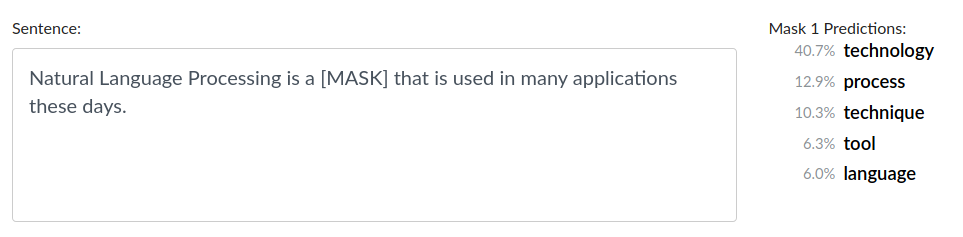
\includegraphics[width=\textwidth]{figures/bertallen.png}
    \url{https://demo.allennlp.org/masked-lm}
\end{frame}

\begin{frame}{What do they learn?}
    \begin{itemize}
        \item Depends on the model's neural network architecture.
        \item Various research studies showed that such contextual representations learn different kinds of syntactic properties (even though they are not explicitly trained for that).
        \item "probing" models to understand what they learn is an active area of research in NLP now. 
    \end{itemize}
\end{frame}

\begin{frame}{How can we use these learned representations?}
    \begin{itemize}
        \item As feature extractors: instead of using static embeddings, or BOW/TF-IDF or hand crafted representations, these representations can directly be used as features for downstream tasks such as text classification, information extraction etc. \pause
        \item For fine-tuning: start with these representations (which were learnt from training on language modeling tasks) and let a neural network "tune" them to suit the current task (e.g., text classification). 
    \end{itemize}
\end{frame}

\begin{frame}{What is fine-tuning?}
\begin{itemize}
    \item The representations learned from training a BERT model can be used as inputs/features to any other task (e.g., text classification)
    \item When we are using a neural network to learn this task, it transforms these input representations to suit that particular task. 
    \item The pre-trained model's weights are then altered ("fine-tuned") while training for the task i.e., this pre-trained architecture is then "retrained" to suit this task. 
\end{itemize}\end{frame}

\begin{frame}{What is happening during fine-tuning?}
\framesubtitle{Let us start with "before" fine-tuning}
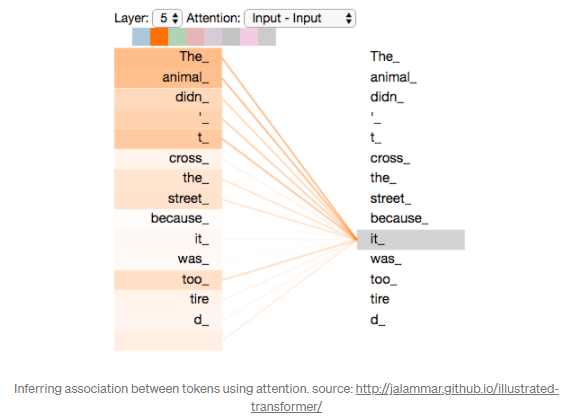
\includegraphics[width=\textwidth]{figures/attention.png}
\end{frame}

\begin{frame}{What happens during fine-tuning?}
\framesubtitle{A case study of using BERT to fine tune "aspect based sentiment analysis"}
    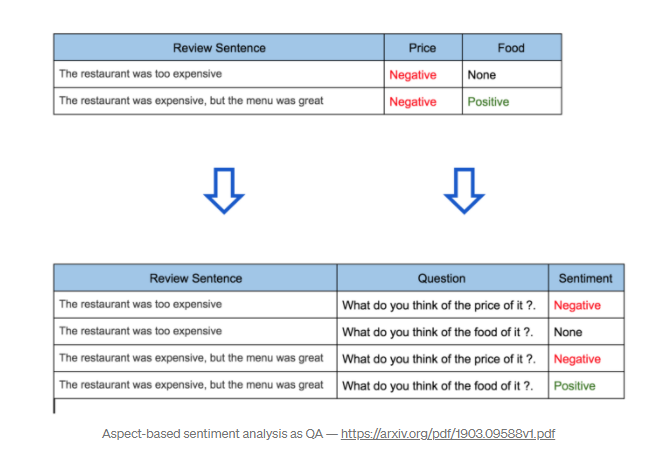
\includegraphics[width=0.8\textwidth]{figures/aspect.png}
    \href{https://towardsdatascience.com/what-does-a-fine-tuned-bert-model-look-at-2eb39b6868dd}{"What does a fine-tuned bert model look at?"}
\end{frame}

\begin{frame}{What happens during fine-tuning?}
    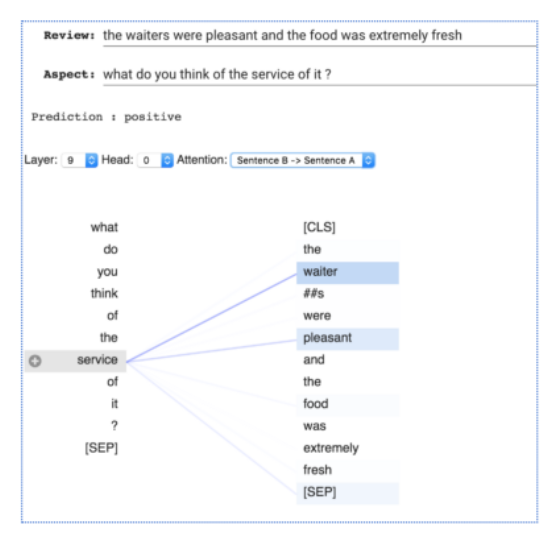
\includegraphics[width=0.7\textwidth]{figures/aspect2.png}
    \href{https://towardsdatascience.com/what-does-a-fine-tuned-bert-model-look-at-2eb39b6868dd}{"What does a fine-tuned bert model look at?"}
\end{frame}

\begin{frame}{What happens during fine-tuning?}
    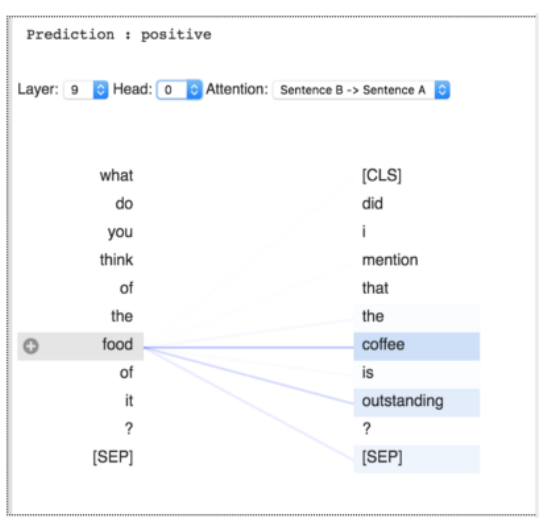
\includegraphics[width=0.7\textwidth]{figures/aspect3.png}
    \href{https://towardsdatascience.com/what-does-a-fine-tuned-bert-model-look-at-2eb39b6868dd}{"What does a fine-tuned bert model look at?"}
\end{frame}

\begin{frame}{Does this really work in practice?}
\framesubtitle{A small exercise}
    Go to your breakout rooms, and browse through the BERT based demos at: \url{https://demos.pragnakalp.com/}. Pick one of them, and play with it for sometime (10 minutes). When you back, each team can share their observations.
\end{frame}

\begin{frame}{}
    Share your observations. 
\end{frame}

\begin{frame}{Beyond the original BERT}
\begin{itemize}
    \item Improvements to model architecture  (e.g., RoBERTa)
    \item Language specific BERT models (e.g., CamemBERT)
    \item Multilingual BERT models (e.g., mBERT)
    \item Compressed BERT (e.g., DistillBERT)
\end{itemize}
..... 
\end{frame}

\begin{frame}{Things to keep in mind}
\begin{itemize}
    \item It is expensive and resource intensive to train your own BERT or any other such language model. \item "Training GPT-3 would cost over \$4.6M using a Tesla V100 cloud instance." (\href{https://lambdalabs.com/blog/demystifying-gpt-3/}{source})
    \item Using the pre-trained model + fine tuning it is how it is used in general purpose cases.
    \item However, even the pre-trained models are super large, and fine-tuning can also get resource intensive (and there may be challenges with deploying these). \pause
    \item DistillBERT and other such recent developments address this problem to some extent. 
\end{itemize}    
\end{frame}

\begin{frame}{}
    \Large Using embedding representations for text classification - examples
    
    \href{https://github.com/practical-nlp/practical-nlp/tree/master/Ch4}{Source: Chapter 4 of Practical NLP book (its Github repo, that is)}
\end{frame}

\begin{frame}{Using word2vec}
    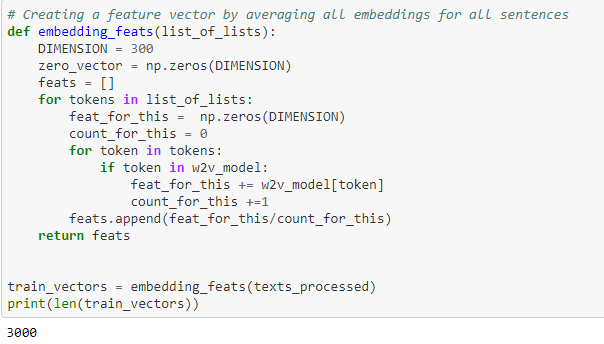
\includegraphics[width=\textwidth]{figures/w2vfeatextractor.PNG}
    (\href{https://github.com/practical-nlp/practical-nlp/blob/master/Ch4/03_Word2Vec_Example.ipynb}{full code})
\end{frame}

\begin{frame}{Then what?}
    \begin{itemize}
        \item Once you extracted these features, it is the same as any other classification example we saw in earlier classes. 
        \item Note: In this example, we used  gensim (in the textbook).
        \item But the same representation can be obtained with a one liner in spacy (without having to write the document level aggregation code).
    \end{itemize}
\end{frame}

\begin{frame}[fragile]{using FastText}
\tiny
    \begin{verbatim}
from fasttext import train_supervised 
model = train_supervised(input=train_file, label="__class__", 
                         lr=1.0, epoch=75, loss='ova', 
                         wordNgrams=2, dim=200, thread=2, 
                         verbose=100)
                         
results = model.test(test_file,k=1)
print(f"Test Samples: {results[0]} Precision : {results[1]*100:2.4f} Recall: {results[2]*100:2.4f}")
    \end{verbatim}
    (\href{https://github.com/practical-nlp/practical-nlp/blob/master/Ch4/04_FastText_Example.ipynb}{Full code})
\end{frame}

\begin{frame}{What's different?}
    \begin{itemize}
        \item fasttext library itself natively supports classification task.
        \item It is also blazing fast. So, for larger datasets, where something like logistic regression may take forever to train, fasttext trains within a minute. 
    \end{itemize}
\end{frame}

\begin{frame}[fragile]{Training Doc2Vec (my favorite even in BERT era)}
\tiny
    \begin{verbatim}
#prepare training data in doc2vec format:
train_doc2vec = [TaggedDocument((d), tags=[str(i)]) 
                for i, d in    enumerate(train_data)]
#Train a doc2vec model to learn tweet representations. 
model = Doc2Vec(vector_size=50, alpha=0.025, 
               min_count=5, dm =1, epochs=100)
model.build_vocab(train_doc2vec)
model.train(train_doc2vec, 
            total_examples=model.corpus_count, 
            epochs=model.epochs)
model.save("d2v.model")
print("Model Saved")
    \end{verbatim}
        (\href{https://github.com/practical-nlp/practical-nlp/blob/master/Ch4/02_Doc2Vec_Example.ipynb}{Source code})
\end{frame}

\begin{frame}[fragile]{Using Doc2Vec}
    \tiny
    \begin{verbatim}
#Infer the feature representation for training and test data using the trained model
model= Doc2Vec.load("d2v.model")
#infer in multiple steps to get a stable representation. 
train_vectors =  [model.infer_vector(list_of_tokens, steps=50) 
                  for list_of_tokens in train_data]
test_vectors = [model.infer_vector(list_of_tokens, steps=50) 
                for list_of_tokens in test_data]

#Use any regular classifier like logistic regression
from sklearn.linear_model import LogisticRegression
myclass = LogisticRegression(class_weight="balanced") 
#because classes are not balanced in training data!
myclass.fit(train_vectors, train_cats)
preds = myclass.predict(test_vectors)
print(classification_report(test_cats, preds))
    \end{verbatim}
    (\href{https://github.com/practical-nlp/practical-nlp/blob/master/Ch4/02_Doc2Vec_Example.ipynb}{Source code})
\end{frame}

\begin{frame}[fragile]{using BERT: no fine tuning}
\tiny
    \begin{verbatim}
    from transformers import AutoTokenizer, AutoModel, pipeline
    model = "bert-base-uncased" 
    #all models at: https://huggingface.co/models
    model = AutoModel.from_pretrained(modelpath)
    tokenizer = AutoTokenizer.from_pretrained(modelpath)
    nlp = pipeline('feature-extraction')
    sample_text = "This is a sample sentence"
    feat_vector = nlp(sample_text)[0][0]
    \end{verbatim}
    - do this for all your training data, and use it with some classifier!
\end{frame}

\begin{frame}{BERT: fine-tuning}
    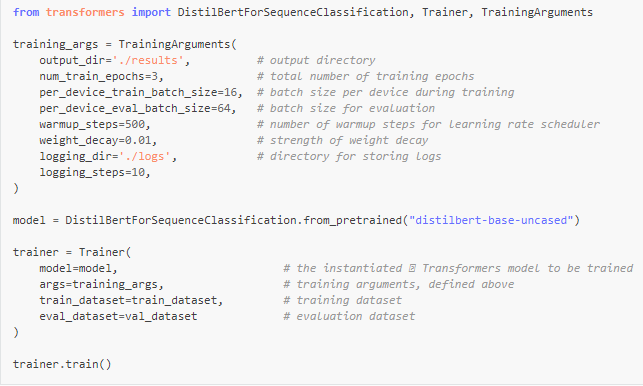
\includegraphics[width=\textwidth]{figures/huggingfacetuning.PNG}
    \tiny source: \url{https://huggingface.co/transformers/custom_datasets.html}
\end{frame}

\begin{frame}[fragile]{BERT: fine-tuning}
\framesubtitle{Save and use this model}
    \tiny
    \begin{verbatim}
      save_directory = "/saved_models"
      model.save_pretrained(save_directory)
      tokenizer.save_pretrained(save_directory) 
      
      loaded_tokenizer = DistilBertTokenizer.from_pretrained(save_directory)
       loaded_model = TFDistilBertForSequenceClassification.from_pretrained(save_directory)
       
       predict_input = loaded_tokenizer.encode(test_text,
                                 truncation=True,
                                 padding=True,
                                 return_tensors="tf")

        output = loaded_model(predict_input)[0]

       prediction_value = tf.argmax(output, axis=1).numpy()[0]
    \end{verbatim}
    \href{https://www.sunnyville.ai/fine-tuning-distilbert-multi-class-text-classification-using-transformers-and-tensorflow/}{Source Code}
\end{frame}

\begin{frame}{BERT: fine-tuning - other options}
    In our book, we showed fine-tuning before hugging face's simple interface was released. Two examples are below:
    \begin{enumerate}
        \item \href{https://github.com/practical-nlp/practical-nlp/blob/master/Ch4/07_BERT_Sentiment_Classification_IMDB_ktrain.ipynb}{Using ktrain, a light weight deep learning library}
        \item \href{https://github.com/practical-nlp/practical-nlp/blob/master/Ch4/06_BERT_IMDB_Sentiment_Classification.ipynb}{using keras and pytorch}
    \end{enumerate}
\end{frame}

\begin{frame}{Other useful things todo}
    \begin{itemize}
        \item Visualizing embeddings (using tools such as t-sne, bertviz etc) to understand what the models are learning.
        \item Interpreting model predictions (using tools such as LIME, SHAP, Anchors etc) and explaining why a prediction was made by the model
    \end{itemize}
\end{frame}

\begin{frame}{Resources for learning further:}
    \begin{itemize}
        \item \href{https://sites.google.com/view/embeddings-in-nlp/}{"Embeddings in NLP"} book and recent (Dec 2020) tutorial at COLING 2020 (video is in the website)
        \item \href{https://web.stanford.edu/~jurafsky/slp3/6.pdf}{Chapters 6}, \href{https://web.stanford.edu/~jurafsky/slp3/7.pdf}{7} in "Speech and Language Processing" 3rdEdition
        \item \href{http://jalammar.github.io/}{"Illustrated *" posts by Jay Alammar}
        \item \href{https://arxiv.org/abs/2002.12327}{A Primer in BERTology: What we know about how BERT works}
    \end{itemize}
\end{frame}

\begin{frame}
\frametitle{Plan for Friday's class}
\begin{itemize}
\item Teams presenting:
\begin{itemize}
    \item Yixuan, Kuan and Ting-Yu: "The Multilingual Amazon Reviews Corpus".
    \item Nelly and Hebah: " Data augmentation using machine translation for fake news detection in the Urdu language."
    \item Leyre, Lorena, Mourhaf and Siena: " Contextual word representations: putting words into computers".
\end{itemize}
\item Rest of the time: I will try to summarize a some relevant stuff to the papers presented, which I think is useful for you.
\item Potentially: Some group exercises.
\end{itemize}
\end{frame}

\end{document}

\begin{frame}
\frametitle{Last Class}
\begin{itemize}
\item 
\end{itemize}
\end{frame}
